\documentclass{article}

\usepackage{arxiv}

\usepackage[utf8]{inputenc}
\usepackage[T1]{fontenc}
\usepackage[brazilian]{babel}
\usepackage[hidelinks,hypertexnames=false]{hyperref}
\usepackage{url}
\usepackage{graphicx}
\usepackage{booktabs}
\usepackage{amsmath, amssymb}
\usepackage{microtype}
\usepackage{placeins}
\usepackage{float}

\usepackage{natbib}
\bibliographystyle{unsrtnat}

\title{Comparação entre SVM supervisionada e One-Class SVM para detecção inter-paciente de anomalias em batimentos ECG}

\author{
  Juliano Eleno Silva Pádua\thanks{E-mail \texttt{julianopadua@estudante.ufscar.br}.}\\
  Grupo 6, Processamento Digital de Sinais\\
  Universidade Federal de São Carlos
  \And
  Pedro Arthur Verger Paulino\thanks{E-mail \texttt{pedropaulino@estudante.ufscar.br}.}\\
  Grupo 6, Processamento Digital de Sinais\\
  Universidade Federal de São Carlos
  \And
  Matheo Sebastian Duarte Davalos\thanks{E-mail \texttt{matheo@estudante.ufscar.br}.}\\
  Grupo 6, Processamento Digital de Sinais\\
  Universidade Federal de São Carlos
  \AND
  Ricardo Jose Ferrari\thanks{E-mail \texttt{rferrari@ufscar.br}.}\\
  Docente da disciplina\\
  Universidade Federal de São Carlos
}

\begin{document}

\maketitle

\begin{abstract}
A comparação entre detectores one-class para batimentos ECG anômalos exige
avaliar, no mesmo protocolo, como a escolha do algoritmo responde a
representações progressivamente mais ricas do sinal e a diferentes custos de
inferência. A análise usa a MIT-BIH Arrhythmia Database em formato WFDB, com
canal MLII, janelas centradas nas anotações de batimento, separação
inter-paciente e treinamento restrito a batimentos normais. O protocolo rotula
batimentos \texttt{N} como normais e demais símbolos válidos não-paced como
anomalias apenas na etapa de avaliação. Quatro estágios cumulativos organizam a
engenharia de features, partindo de descritores morfológicos e intervalo RR no
sinal bruto, seguindo para o sinal filtrado por FIR, depois para descritores
espectrais e STFT, e por fim para respostas de filtros de Gabor 1D em janelas
aproximadas P, QRS e T. One-Class SVM, Isolation Forest e Local Outlier Factor
em modo novelty são comparados com foco em métricas adequadas ao
desbalanceamento, sobretudo PR-AUC, além de ROC-AUC, precision, recall,
F1-score, matriz de confusão e tempo de escore por batimento. Os resultados
preliminares indicam comportamento não monotônico entre algoritmos e estágios
de representação, com variações de desempenho que dependem da interação entre
detector e conjunto de features. A comparação fornece uma base reprodutível
para discutir quais abordagens one-class são mais competitivas nesse cenário e
qual par representação-detector oferece melhor compromisso entre separação de
anomalias e custo computacional.

\end{abstract}

\section{Introdução}
O eletrocardiograma reúne informação morfológica, rítmica e espectral em uma
série temporal curta e biologicamente estruturada. Um protocolo automático que
pretende separar batimentos normais de batimentos anômalos precisa preservar o
alinhamento com o R-peak, estabilizar a linha de base e produzir descritores
que continuem legíveis depois da classificação. A MIT-BIH Arrhythmia Database
permanece adequada para esse objetivo por oferecer sinais reais, anotações
públicas e acesso padronizado por WFDB
\citep{moody2001mitdb,goldberger2000physionet,wfdb2022software}.

Morfologia de batimento e intervalos RR seguem entre os descritores mais
interpretáveis em estudos com separação inter-paciente entre treino e teste
\citep{dechazal2004heartbeat,doquire2011featureselection,mousavi2019inter}. O
interesse aqui não é apenas medir uma acurácia global, mas organizar uma
representação compacta que preserve a fisiologia do traçado filtrado e permita
comparar dois regimes de treinamento sob o mesmo vetor de entrada. Por essa
razão, nenhuma feature é extraída do sinal bruto. Toda a modelagem parte de um
ECG previamente filtrado e alinha descritores morfológicos, contexto RR,
informação espectral e respostas Gabor localizadas em regiões aproximadas de P,
QRS e T.

A comparação entre SVM supervisionada e One-Class SVM surge de uma assimetria
recorrente em dados biomédicos. A formulação supervisionada explora exemplos
normais e anômalos no ajuste e funciona como referência para o que o mesmo
conjunto de features consegue oferecer quando há rótulos completos. A
formulação one-class, em contraste, aprende apenas a distribuição dos
batimentos normais e testa se o afastamento dessa região já basta para ranquear
anomalias \citep{cortes1995support,scholkopf2001support,pimentel2014novelty}.
As duas leituras respondem a perguntas diferentes, e a distância entre elas
deve ser interpretada como diferença de informação disponível no treino, não
apenas como troca de algoritmo.

O recorte permanece binário e metodológico. O protocolo não diagnostica classes
clínicas específicas nem tenta reproduzir um fluxo hospitalar completo. O
rótulo \texttt{N} representa normalidade, enquanto os demais símbolos válidos
de batimento entram como anomalia apenas para avaliação. Essa redução concentra
a análise na pergunta de DSP e evita misturar o estudo com classificação
multi-classe de arritmias.

A representação final foi consolidada a partir do notebook do grupo e reúne 18
features filtradas, com seis descritores morfológicos, três features rítmicas,
quatro descritores espectrais e cinco respostas Gabor. A pergunta central passa
a ser direta. Dado esse vetor final, até que ponto a SVM supervisionada e a
One-Class SVM mantêm desempenho útil no split inter-paciente DS1-DS2.

A PR-AUC ocupa o papel central porque a classe anômala é minoritária e o custo
de falsos positivos aparece diretamente na precision \citep{davis2006prroc}.
ROC-AUC, recall, F1 e matrizes de confusão entram como leitura complementar do
regime operacional. O objetivo, portanto, é comparar os dois modelos sob a
mesma representação filtrada final e verificar quanto da separação inter-
paciente depende do acesso prévio a anomalias no treino.


\section{Fundamentação teórica}
\label{sec-theory}

\subsection{ECG, morfologia e segmentação}

Um batimento ECG típico apresenta onda P, complexo QRS e onda T. A anotação de
batimento na MIT-BIH fornece uma referência temporal associada ao evento
cardíaco, usada no protocolo como centro da janela de extração. A
Figura~\ref{fig-ecg-schema} mostra as regiões fisiológicas aproximadas usadas
para organizar as features locais.

\begin{figure}[!htbp]
  \centering
  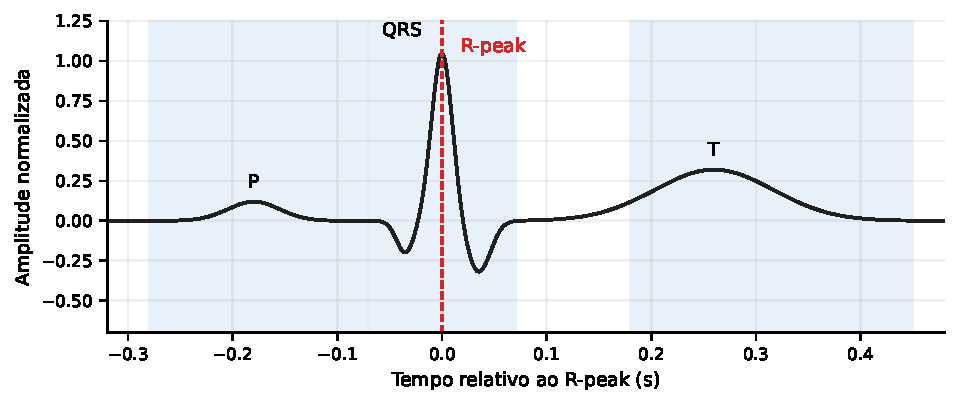
\includegraphics[width=0.95\linewidth]{figures/fig_ecg_waves_schema.pdf}
  \caption{Batimento ECG com onda P, complexo QRS, onda T, R-peak e janelas
  aproximadas usadas na extração de features.}
  \label{fig-ecg-schema}
\end{figure}

\subsection{Filtragem FIR}

Registros ambulatoriais de ECG podem conter deriva de linha de base,
interferência de rede e ruído de alta frequência. A literatura de
monitoramento e detecção de QRS sustenta o uso de bandas reduzidas quando a
pergunta depende sobretudo da morfologia do batimento e da localização do
complexo QRS. Thakor et al. mostraram que um passa-faixa centrado próximo de
17 Hz melhora a razão sinal-ruído do QRS em relação a T, ruído muscular e
interferência de rede \citep{thakor1984qrs}. Elgendi et al. analisaram sinais
da MIT-BIH e indicaram que a faixa de 0,5 a 40 Hz preserva componentes centrais
do QRS em aplicações de detecção e processamento eficiente
\citep{elgendi2017efficient}. O protocolo usa, portanto, uma cadeia FIR
passa-faixa de 0,5 a 40 Hz com janela de Hamming e aplicação forward-backward
em fase zero. O rejeita-faixa em 60 Hz não é mantido, pois a própria etapa
passa-baixa já remove a interferência de rede fora da banda preservada. O ganho
dessa etapa é medido pela comparação entre \texttt{A0 raw} e
\texttt{A1 filtered}, sem pressupor melhora automática na detecção.

\subsection{STFT e filtros de Gabor}

Estruturas do ECG ocupam escalas temporais distintas. O complexo QRS é curto e
concentra componentes relativamente rápidas, enquanto P e T tendem a aparecer
em janelas mais largas e suaves. A STFT resume energia local em janelas curtas;
filtros de Gabor 1D representam o sinal por átomos localizados no tempo e na
frequência \citep{gabor1946theory}. Essa família já foi usada para extrair
features de ECG em combinação com STFT e modelos gaussianos
\citep{lee2012gabor}, e transformadas de Gabor de Q constante aparecem em
representações tempo-frequência recentes para diagnóstico automático em ECG
\citep{eltrass2021cqgabor}. Para um sinal discreto \(x[n]\), a STFT pode ser
escrita como

\[
X(m, \omega)=\sum_n x[n]w[n-m]e^{-j\omega n},
\]

em que \(w\) define a janela temporal local. Os filtros de Gabor usados como
features seguem a ideia de uma portadora senoidal modulada por uma envoltória
gaussiana,

\[
g_{f,\sigma}(t)=e^{-t^2/(2\sigma^2)}\cos(2\pi f t).
\]

A entrada das features Gabor apenas em \texttt{A3} isola sua contribuição em
relação a morfologia, RR e espectro. Para evitar uma expansão excessiva da
dimensionalidade, o banco é definido por região fisiológica aproximada. A
janela P usa frequência central de 7 Hz, o QRS usa 15 Hz e a janela T usa
5 Hz, com três ciclos no envelope gaussiano. A escolha acompanha a leitura
fisiológica de P e T como eventos mais lentos e largos que o QRS, enquanto a
frequência do QRS permanece próxima da região de maior separação espectral
descrita por Thakor et al. \citep{thakor1984qrs}. As respostas real e
imaginária são combinadas em magnitude, reduzindo a dependência da fase local
do complexo.

\subsection{Detecção one-class}

One-Class SVM estima uma região de suporte para dados normais
\citep{scholkopf2001support}. A formulação primal busca separar os exemplos
normais da origem no espaço de features,

\[
\min_{w,\rho,\xi}\frac{1}{2}\|w\|^2+\frac{1}{\nu n}\sum_i \xi_i-\rho
\quad
\text{sujeito a}
\quad
w^\top\phi(x_i)\geq\rho-\xi_i,\ \xi_i\geq0.
\]

Isolation Forest atribui maior anomalia a pontos isolados por menos
particionamentos aleatórios \citep{liu2008isolation}. O escore depende do
comprimento esperado do caminho \(E[h(x)]\) nas árvores,

\[
s(x,n)=2^{-E[h(x)]/c(n)}.
\]

Local Outlier Factor compara a densidade de uma amostra com a densidade de seus
vizinhos \citep{breunig2000lof}. A densidade de alcançabilidade local e o fator
LOF podem ser resumidos por

\[
\operatorname{lrd}_k(p)=
\left(
\frac{1}{|N_k(p)|}
\sum_{o\in N_k(p)}\operatorname{reachdist}_k(p,o)
\right)^{-1}
\]

e

\[
\operatorname{LOF}_k(p)=
\frac{1}{|N_k(p)|}
\sum_{o\in N_k(p)}
\frac{\operatorname{lrd}_k(o)}{\operatorname{lrd}_k(p)}.
\]

No scikit-learn, o uso de LOF para novelty detection requer
\texttt{novelty=True} e avaliação em dados diferentes dos dados usados no
ajuste \citep{sklearnNovelty}.

\subsection{Custo computacional e inferência}

A comparação de detectores também depende do custo necessário para transformar
um batimento em decisão. Pimentel et al. tratam eficiência como parte da
aplicabilidade de métodos de novelty detection, especialmente quando o modelo de
normalidade precisa operar sobre muitos exemplos de teste
\citep{pimentel2014novelty}. Isolation Forest foi proposto com complexidade
linear e baixo uso de memória por subamostragem, enquanto LOF depende de
consultas a vizinhos e pode ficar mais sensível ao crescimento dimensional
\citep{liu2008isolation,breunig2000lof}. Em aplicações de monitoramento
contínuo, a literatura de edge computing motiva processar dados perto da fonte
quando tempo de resposta, energia e transmissão são restrições relevantes
\citep{shi2016edge}.

\subsection{Avaliação inter-paciente e dados desbalanceados}

A separação entre pacientes reduz avaliações otimistas causadas por
similaridade intra-paciente. Por esse motivo, a divisão DS1 e DS2 usada em
estudos com MIT-BIH orienta o protocolo experimental
\citep{mousavi2019inter}. A PR-AUC recebe prioridade narrativa porque anomalias
são minoria e a curva precision-recall responde diretamente à quantidade de
falsos positivos entre os casos sinalizados \citep{davis2006prroc}.


\section{Metodologia}
\label{sec-methodology}

\subsection{Base, canal e protocolo de rótulos}

A MIT-BIH Arrhythmia Database reúne registros ambulatoriais de cerca de
30 minutos, amostrados a 360 Hz em dois canais
\citep{moody2001mitdb,physionetmitdb}. O pipeline lê os arquivos locais com
WFDB, prioriza o canal MLII quando disponível e usa as anotações \texttt{atr}
como referência temporal dos batimentos. Após a exclusão dos registros
paced-heavy \texttt{102}, \texttt{104}, \texttt{107} e \texttt{217}, o
protocolo mantém 44 registros.

O rótulo binário é usado apenas na avaliação. Batimentos \texttt{N} formam a
classe normal, enquanto os demais símbolos válidos de batimento formam a classe
anômala. Símbolos técnicos, mudanças de ritmo e batimentos paced ficam fora da
amostra analisável. Essa escolha preserva o foco em anomalias de batimento
não-paced e evita transformar o benchmark em um detector de marcapasso.

\subsection{Segmentação e filtragem do sinal de entrada}

Cada linha experimental corresponde a uma janela de 0,25 s antes e 0,45 s
depois da anotação. Janelas que encostam nas bordas do registro são descartadas
para preservar duração constante. O sinal é filtrado no registro completo antes
da segmentação, pois aplicar \texttt{filtfilt} diretamente em janelas curtas
introduziria artefatos de borda.

A cadeia adotada remove primeiro a média do registro e, em seguida, aplica dois
filtros FIR lineares com janela de Hamming e fase zero por forward-backward. O
primeiro é um passa-alta em 0,5 Hz com largura de transição de 1 Hz e
1189 coeficientes. O segundo é um passa-baixa em 40 Hz com largura de
transição de 8 Hz e 149 coeficientes. A escolha combina preservação da
morfologia útil do ECG com atenuação de deriva de linha de base, ruído muscular
e componentes de alta frequência \citep{thakor1984qrs,elgendi2017efficient,butt2020signalpiloted}.
Como o R-peak serve de âncora para a segmentação e para as janelas fisiológicas
de P, QRS e T, a filtragem em fase zero evita deslocamentos temporais que
prejudicariam a interpretação local do batimento.

Nenhuma feature é extraída do sinal bruto. Todos os descritores do manuscrito
partem desse sinal filtrado comum, o que reduz a influência de ruído residual
na comparação entre os modelos e mantém a base fisiológica da representação.

\begin{figure}[!htbp]
  \centering
  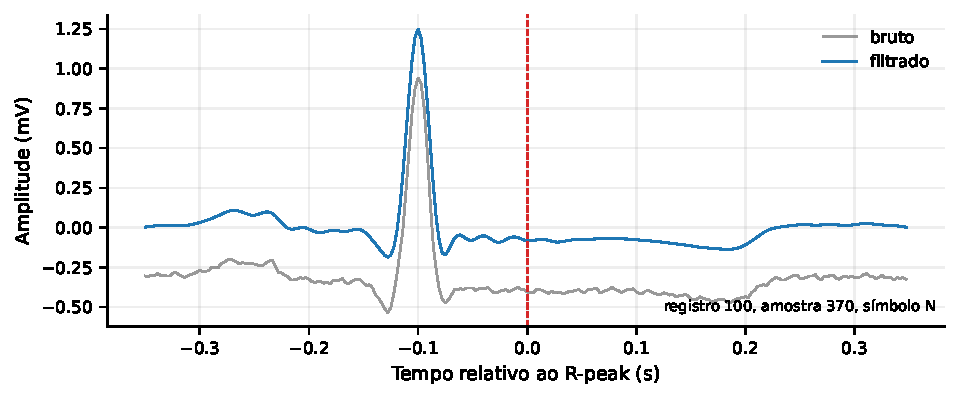
\includegraphics[width=0.95\linewidth]{figures/fig_raw_vs_filtered_beat.pdf}
  \caption{Batimento normal segmentado no mesmo R-peak antes e depois da cadeia FIR.}
  \label{fig-raw-filtered}
\end{figure}

\subsection{Split inter-paciente e tamanho do dataset}

Os registros do grupo DS1 formam o conjunto de treino e os registros DS2 formam
o teste final. Nenhum paciente aparece nos dois lados. Depois da filtragem, da
segmentação e das exclusões, o protocolo produziu 100.694 batimentos válidos.
Desse total, 74.516 pertencem à classe normal e 26.178 à classe anômala. O
treino contém 51.002 batimentos, com 38.088 normais e 12.914 anômalos. O teste
contém 49.692 batimentos, com 36.428 normais e 13.264 anômalos.

\subsection{Representação final do batimento}

O vetor final reúne 18 features e altera apenas a forma de resumir o batimento
filtrado e o seu contexto rítmico local. Não há descritores do sinal bruto nem
expansão massiva de dimensionalidade. A intenção é manter um conjunto compacto,
interpretável e coerente com a segmentação ancorada no R-peak.

\begin{table*}[!htbp]
  \centering
  \caption{Grupos de features da representação final.}
  \label{tab-feature-groups}
  \scriptsize
  \renewcommand{\arraystretch}{1.08}
  \begin{tabular}{lp{8.6cm}r}
    \toprule
    Grupo & Variáveis & Quantidade \\
    \midrule
    Morfologia filtrada & amplitude em R, pico-a-pico, energia, área absoluta, inclinação máxima absoluta e desvio-padrão & 6 \\
    Ritmo & RR anterior, RR posterior e razão RR & 3 \\
    Espectrais & centroide espectral, largura de banda, potência em 8 a 20 Hz e potência em 20 a 40 Hz & 4 \\
    Gabor & energia em P, energia em QRS, máximo em QRS, deslocamento do pico em QRS e energia em T & 5 \\
    \bottomrule
  \end{tabular}
  \renewcommand{\arraystretch}{1.0}
\end{table*}

As features morfológicas resumem amplitude, energia, área absoluta,
variabilidade e inclinação máxima do batimento filtrado. As features rítmicas
capturam o contexto local do intervalo RR antes e depois da batida. Os
descritores espectrais medem quão concentrada ou espalhada está a energia da
janela, com ênfase nas bandas de 8 a 20 Hz e 20 a 40 Hz, associadas a
componentes mais rápidas do QRS. Esse desenho mantém a comparação no domínio do
sinal tratado por DSP e explicita que o vetor final usa morfologia, ritmo,
espectro e respostas locais, não amostras cruas da janela.

\subsection{Banco Gabor do notebook}

A representação final usa exatamente o banco consolidado no notebook do grupo.
A região P recebe um filtro par em 8 Hz com janela de -0,28 s a -0,07 s. A
região QRS recebe um filtro em magnitude em 15 Hz com janela de -0,07 s a
0,07 s. A região T recebe um filtro par em 6 Hz com janela de 0,18 s a 0,45 s.
A Figura~\ref{fig-gabor-bank} mostra os três kernels normalizados, e a
Figura~\ref{fig-gabor-response} ilustra as respostas alinhadas em um batimento
normal e em um batimento anômalo.

\begin{figure}[!htbp]
  \centering
  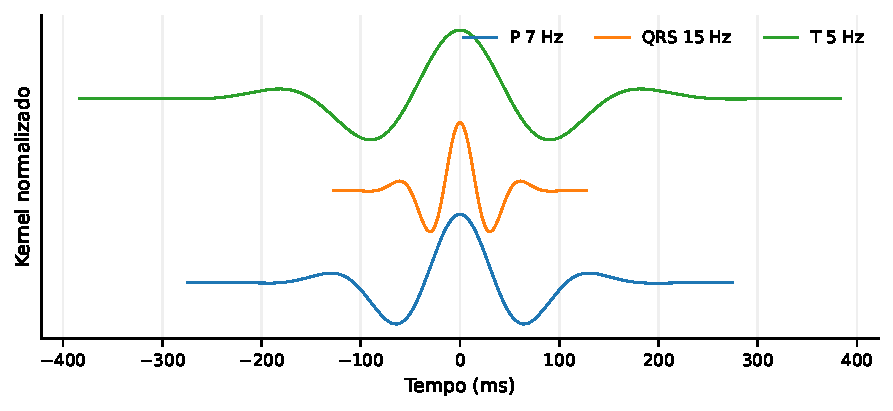
\includegraphics[width=0.95\linewidth]{figures/fig_gabor_filter_bank.pdf}
  \caption{Banco compacto de filtros Gabor 1D usado na representação final.}
  \label{fig-gabor-bank}
\end{figure}

\begin{figure}[!htbp]
  \centering
  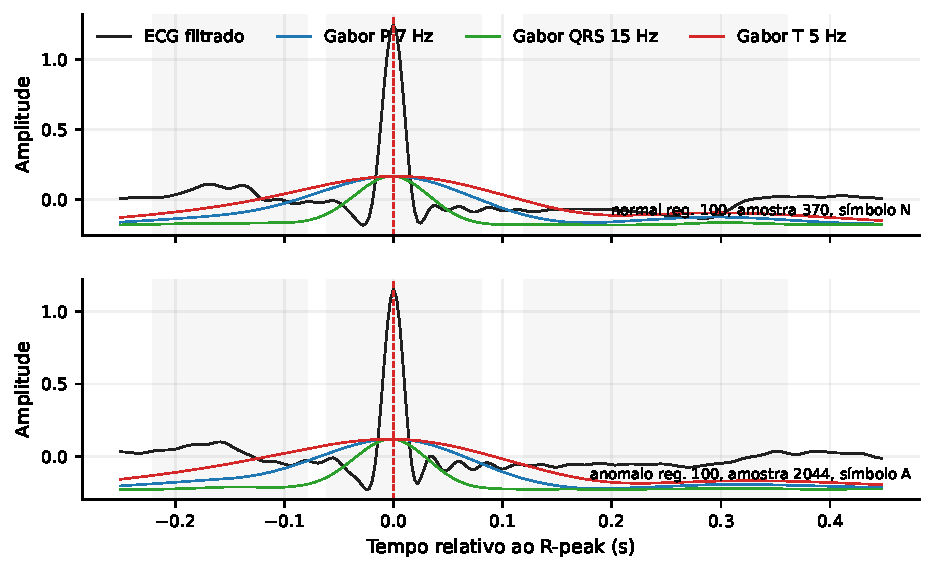
\includegraphics[width=0.95\linewidth]{figures/fig_gabor_response_examples.pdf}
  \caption{Respostas Gabor em um batimento normal e em um batimento anômalo, com janelas aproximadas de P, QRS e T destacadas.}
  \label{fig-gabor-response}
\end{figure}

\subsection{Modelos e métricas}

Dois modelos compartilham a mesma padronização das 18 features, mas usam
regimes de treinamento diferentes. A SVM supervisionada usa kernel RBF,
\texttt{class\_weight=balanced}, \texttt{gamma=scale} e probabilidades
habilitadas. Esse modelo é ajustado com todos os 51.002 batimentos do treino
DS1. A One-Class SVM usa kernel RBF, \texttt{nu=0.05} e
\texttt{gamma=scale}, sendo ajustada apenas com os 38.088 batimentos normais de
DS1.

PR-AUC é a métrica principal. ROC-AUC, precision, recall, F1 e matriz de
confusão complementam a análise. A SVM supervisionada é avaliada pelo escore de
probabilidade da classe anômala, enquanto a One-Class SVM usa o valor negativo
da \texttt{decision\_function}, orientado para que escores maiores representem
maior anomalia.

\begin{figure}[H]
  \centering
  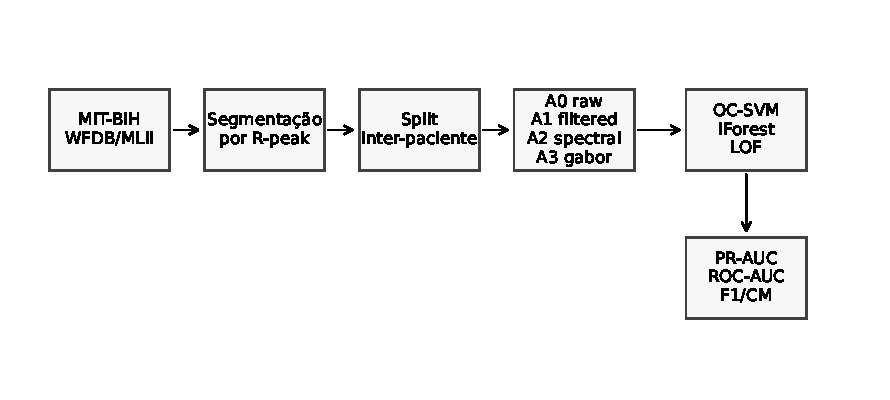
\includegraphics[width=1.0\linewidth]{figures/fig_pipeline_ablation.pdf}
  \caption{Pipeline experimental resumido.}
  \label{fig-pipeline}
\end{figure}
\FloatBarrier


\section{Resultados}
\label{sec-results}

A execução completa gerou a representação final de 18 features para 100.694
batimentos válidos. A SVM supervisionada foi treinada com os 51.002 batimentos
de DS1, enquanto a One-Class SVM recebeu apenas os 38.088 batimentos normais
desse mesmo conjunto. O teste em DS2 manteve 49.692 batimentos, com
36.428 normais e 13.264 anômalos. A
Tabela~\ref{tab-final-metrics} resume a comparação principal.

\begin{table*}[!htbp]
  \centering
  \caption{Resultados da comparação inter-paciente para a representação final.}
  \label{tab-final-metrics}
  \small
  \renewcommand{\arraystretch}{1.10}
  \begin{tabular}{lp{3.8cm}rrrrrr}
    \toprule
    Modelo & Treino & Features & PR-AUC & ROC-AUC & Precision & Recall & F1 \\
    \midrule
    SVM supervisionada & normais + anômalos de DS1 & 18 & 0.528 & 0.748 & 0.485 & 0.358 & 0.412 \\
    One-Class SVM & apenas normais de DS1 & 18 & 0.448 & 0.537 & 0.354 & 0.388 & 0.370 \\
    \bottomrule
  \end{tabular}
  \renewcommand{\arraystretch}{1.0}
\end{table*}

A SVM supervisionada superou a One-Class SVM em PR-AUC, ROC-AUC, precision e
F1 na mesma representação final. A diferença de 0,080 ponto de PR-AUC mostra
vantagem consistente do regime supervisionado quando há rótulos anômalos
disponíveis no treino. A Figura~\ref{fig-pr-curves} mostra que essa vantagem
não depende apenas de um limiar específico, pois a SVM mantém precision mais
alta ao longo da maior parte da faixa de recall observada.

\begin{figure}[H]
  \centering
  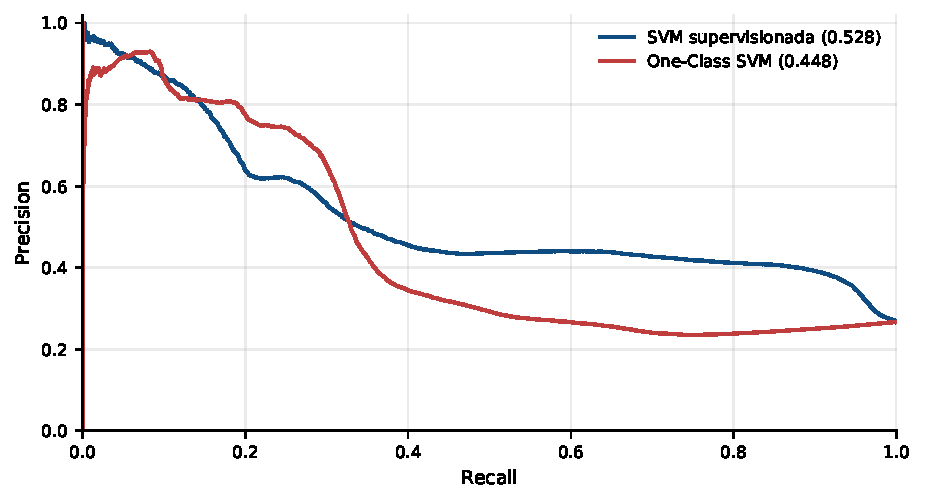
\includegraphics[width=0.72\linewidth]{figures/fig_model_precision_recall.pdf}
  \caption{Curvas precision-recall da SVM supervisionada e da One-Class SVM no teste inter-paciente.}
  \label{fig-pr-curves}
\end{figure}

O limiar operacional destaca um trade-off diferente entre os modelos. A
One-Class SVM recuperou 5153 anomalias no teste, enquanto a SVM supervisionada
recuperou 4753. Esse ganho de 400 verdadeiros positivos veio acompanhado de
4379 falsos positivos adicionais. A queda de precision para 0,354, frente a
0,485 na SVM supervisionada, confirma que a fronteira one-class operou de forma
mais permissiva no conjunto inter-paciente.

\begin{table}[H]
  \centering
  \caption{Matrizes de confusão no teste inter-paciente.}
  \label{tab-confusion-matrices}
  \small
  \renewcommand{\arraystretch}{1.10}
  \begin{tabular}{lrrrr}
    \toprule
    Modelo & TN & FP & FN & TP \\
    \midrule
    SVM supervisionada & 31385 & 5043 & 8511 & 4753 \\
    One-Class SVM & 27006 & 9422 & 8111 & 5153 \\
    \bottomrule
  \end{tabular}
  \renewcommand{\arraystretch}{1.0}
\end{table}

\begin{figure}[H]
  \centering
  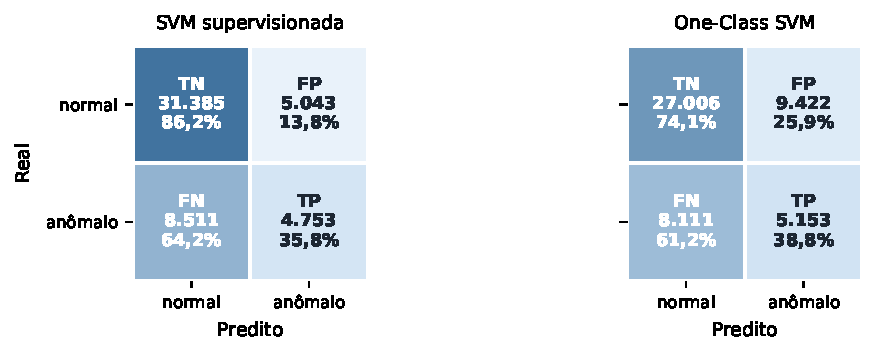
\includegraphics[width=0.84\linewidth]{figures/fig_confusion_matrices.pdf}
  \caption{Matrizes de confusão visualizadas por proporção em cada classe real. Cada célula mostra o tipo de acerto ou erro, a contagem e o percentual da linha correspondente.}
  \label{fig-confusion-heatmaps}
\end{figure}

As matrizes de confusão da Tabela~\ref{tab-confusion-matrices} e da
Figura~\ref{fig-confusion-heatmaps} tornam esse contraste mais direto. Entre os
batimentos normais, a SVM supervisionada manteve 86,2\% classificados como
normais, contra 74,1\% na One-Class SVM. Entre os batimentos anômalos, a
One-Class SVM reconheceu 38,8\%, contra 35,8\% na SVM supervisionada. A pequena
vantagem de recall da formulação one-class veio acompanhada de perda expressiva
de especificidade.
\FloatBarrier


\section{Discussão}
A comparação entre A0 e A1 mostra que a filtragem FIR não deve ser tratada como
sinônimo de melhora na detecção. A remoção de componentes lentas e de
interferência pode tornar a morfologia mais regular, mas também altera sinais
estatísticos que alguns detectores exploram. O One-Class SVM perdeu PR-AUC após
a filtragem, enquanto Isolation Forest e LOF melhoraram. Essa divergência indica
que a qualidade visual do sinal e a separabilidade para um detector one-class
não são propriedades equivalentes.

A entrada de descritores espectrais em A2 favoreceu principalmente Isolation
Forest. Uma interpretação plausível é que energia por bandas, frequência
dominante e estatísticas de STFT criam partições úteis para árvores aleatórias,
sobretudo quando anomalias se afastam por concentração de energia em faixas
específicas. O mesmo acréscimo reduziu o PR-AUC do LOF em relação a A1, o que
sugere perda de estrutura local útil ou aumento de dispersão em dimensões que
não contribuem igualmente para a vizinhança.

As respostas Gabor em A3 produziram o melhor resultado preliminar apenas para
LOF. O padrão é coerente com a hipótese de que energia tempo-frequência
localizada em P, QRS e T pode reorganizar vizinhanças locais de batimentos
normais e anômalos. A mesma representação prejudicou One-Class SVM e Isolation
Forest em relação aos seus melhores estágios, o que recomenda seleção de
features, redução dimensional ou ajuste de hiperparâmetros antes de qualquer
conclusão mais forte sobre Gabor.

A distância entre PR-AUC e métricas em limiar fixo também merece cautela. LOF
atingiu recalls altos com baixa precision, sinalizando grande número de falsos
positivos sob o limiar definido por contaminação. A análise por curva
precision-recall oferece uma leitura mais estável do ranqueamento de anomalias,
enquanto a matriz de confusão depende diretamente de uma escolha operacional de
limiar.

A rotulagem binária normal versus anomalia simplifica classes clínicas com
origens distintas, e as janelas P, QRS e T usadas no protocolo são regiões
aproximadas em torno do R-peak, não delineações clínicas. Ainda assim, a
separação inter-paciente, a exclusão de paced no v1 e o treino restrito a
batimentos normais tornam a primeira execução adequada para uma pergunta de DSP
experimental. O próximo refinamento deve testar sensibilidade a limiares,
seleção de features Gabor e inspeção visual de falsos positivos e falsos
negativos.


\section{Conclusão}
O pipeline experimental permitiu avaliar filtragem FIR, descritores espectrais
e respostas Gabor sob a restrição de treino apenas com batimentos normais. A
execução inter-paciente na MIT-BIH mostrou que o acréscimo de processamento e
features não produz ganho monotônico. One-Class SVM favoreceu a representação
bruta, Isolation Forest respondeu melhor aos descritores espectrais, e LOF teve
seu melhor resultado com features Gabor.

Esses resultados preservam a hipótese como questão experimental, não como
conclusão fechada. A próxima etapa deve concentrar-se em análise de limiar por
FPR alvo, seleção ou compressão de features Gabor, comparação com baselines
supervisionados apenas como referência externa, e inspeção de exemplos de erro.
O enquadramento deve permanecer como benchmark de DSP e detecção one-class, sem
promessa de diagnóstico clínico.


\section*{Agradecimentos}

Os autores reconhecem o uso auxiliar de ferramentas de IA generativa na
preparação do fluxo computacional, organização bibliográfica, depuração,
documentação e revisão linguística. Essas ferramentas não foram tratadas como
fontes de evidência científica, autoridade metodológica ou análise autônoma.

\bibliography{ref}

\end{document}
